\chapter{Implementierung}
\label{ch:implementierung}

\section{Architektur}
\label{sec:architektur}
Die Implementierung der Anwendung besteht aus den folgenden Komponenten, die in \autoref{fig:architektur} dargestellt sind:
\begin{figure}[H]
    \centering
    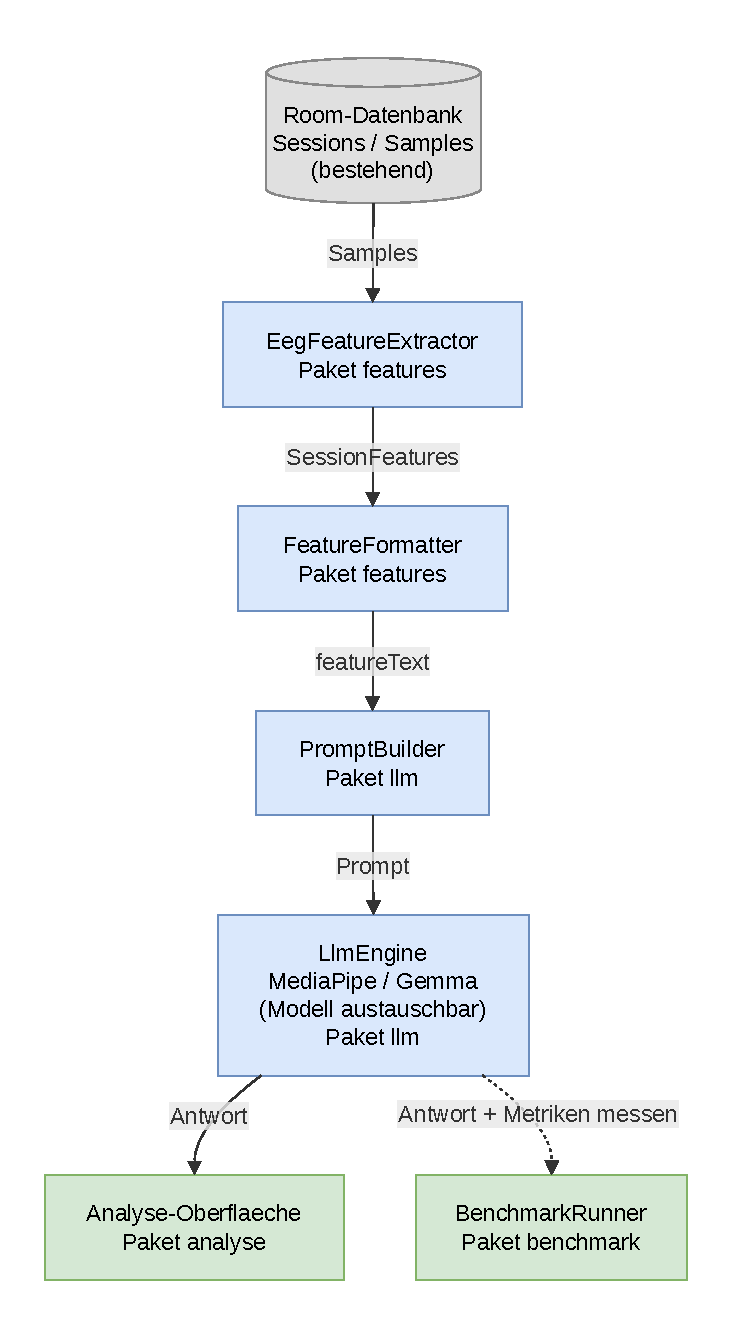
\includegraphics[width=0.6\textwidth]{Graphics/Projektarchitektur.drawio.pdf}
    \caption{Architektur und Datenfluss der Anwendung \autocite{drawio}}
    \label{fig:architektur}
\end{figure}

\begin{itemize}
\item \textbf{Datenbank:} Der Weg startet über die Datenbank, aus der die Samples abgerufen werden.
\item \textbf{EegFeatureExtractor:} Hier werden die Samples verarbeitet, indem Merkmale berechnet werden.
\item \textbf{FeatureFormatter:} Wandelt die Merkmale in ein für das Sprachmodell verständliches Format um.
\item \textbf{PromptBuilder:} Baut die Anweisung für den Prompt (je Szenario).
\item \textbf{LlmEngine:} Führt das Modell (Gemma via MediaPipe) aus und gibt die Antwort zurück.
\item \textbf{Analyse-Oberfläche:} Zeigt letztlich die Antwort an.
\item \textbf{Benchmark:} Misst die Verarbeitung (Laufzeit, Speicherverbrauch etc.).
\end{itemize}


\noindent Die Architektur ist in drei Kernbereiche unterteilt: zum einen das Paket \texttt{features}, das die Merkmalsextraktion übernimmt; zum anderen das Paket \texttt{llm}, das je nach Szenario den Aufbau des Prompts übernimmt und das Sprachmodell ausführt; und schließlich das Paket \texttt{analyse}, das die Benutzeroberfläche bereitstellt. Durch die Trennung dieser Pakete bleibt der Code übersichtlich, wartbar und erweiterbar.
\medskip

\noindent Ein zentrales Merkmal der Architektur ist die Kapselung des Sprachmodells in der Klasse \texttt{LlmEngine}. Die Klasse stellt eine einfache Schnittstelle bereit, die für das Laden, Anfragen und Freigeben verantwortlich ist. Dadurch wird die konkrete Modell- und Laufzeitumgebung vor dem Rest der Anwendung verborgen. Dies ermöglicht das Austauschen der Modelle, ohne dass die anderen Komponenten angepasst werden müssen.
In dieser Arbeit werden die Modelle Gemma 3 1B und Gemma 2 2B allein durch den Wechsel des Modellpfads auf dem mobilen Gerät geladen. Aus diesem Grund ließe sich an derselben Schnittstelle auch ein anderes Modell anbinden. Möglich wäre es auch, eine andere Laufzeitumgebung oder ein systemintegriertes Modell anzubinden. Diese Entkopplung ermöglicht es, die Anwendung flexibel und ohne großen Aufwand zu erweitern und zu warten.

\noindent Die in \autoref{fig:architektur} grün und blau markierten Komponenten stellen den eigenen Beitrag dar.

\section{Implementierung der Merkmalsextraktion}
\label{sec:impl-features}
Die Merkmalsextraktion ist im Paket \texttt{features} implementiert; zuständig dafür ist die Klasse \texttt{EegFeatureExtractor}. Sie durchläuft für jede Session eine feste Abfolge von Schritten: Als Erstes wird die Session aus der Datenbank geladen, daraufhin wird sie auf ihre Verwertbarkeit geprüft. Anschließend wird sie in gleich große Segmente aufgeteilt, bei denen dann jeweils die spektralen sowie statistischen Merkmale berechnet werden. Die Ergebnisse werden alle im Objekt \texttt{SessionFeatures} gesammelt und schließlich vom \texttt{FeatureFormatter} in einen lesbaren Text umgewandelt, den das Sprachmodell verarbeiten kann. Im Folgenden wird chronologisch auf die einzelnen Schritte genauer eingegangen.
\medskip

\noindent\textbf{Vorbereitung.} Sobald die Klasse erzeugt wird, werden vorab alle wiederverwendbaren Bestandteile angelegt (\autoref{lst:konstruktor}). Dazu gehört das Hann-Fenster, das für die Fourier-Transformation vorab berechnet wird, um bei jedem Fenster nicht erneut erzeugt zu werden. Außerdem wird das FFT-Objekt der Bibliothek JTransforms für die gewählte Fenstergröße instanziiert. Der Standardwert für die Fenstergröße beträgt 256, kann aber variabel angepasst werden. Aus ihr und der Anzahl der Segmente wird die Mindestlänge \texttt{minSamples} der Session berechnet.
\begin{lstlisting}[style=code, caption={Vorberechnung von Hann-Fenster und FFT-Objekt im Konstruktor}, label={lst:konstruktor}]
public EegFeatureExtractor(int windowSize) {
    this.windowSize = windowSize;
    this.hann       = hannWindow(windowSize);
    // Hann-Fenster vorberechnen
    this.fft        = new DoubleFFT_1D(windowSize);
    // FFT-Objekt aus JTransforms
    this.minSamples = windowSize * SEGMENT_COUNT;
}
\end{lstlisting}

\noindent\textbf{Validierung.} Die Methode \texttt{validate} prüft eine Session auf ihre Verwertbarkeit. Es gibt zwei Kriterien, die erfüllt sein müssen. Zum einen muss die Session mindestens so viele Samples enthalten, wie in \texttt{minSamples} berechnet wurde, ansonsten wird \texttt{TOO\_SHORT} zurückgegeben. Zum anderen muss der Anteil ungültiger Samples unter 50\,\% liegen. Ist dies nicht der Fall, wird \texttt{TOO\_MANY\_INVALID} zurückgegeben. Sind beide Kriterien erfüllt, wird die Analyse mit der Rückgabe von \texttt{OK} fortgesetzt, ansonsten wird dem Nutzer eine entsprechende Meldung angezeigt.
\begin{lstlisting}[style=code, caption={Vorabprüfung der Session}, label={lst:validate}]
public enum Check { OK, TOO_SHORT, TOO_MANY_INVALID; }

public Check validate(List<SampleEntity> samples) {
    if (samples == null || samples.size() < minSamples) {
        return Check.TOO_SHORT;
        // zu wenige Samples
    }
    int invalidCount = 0;
    for (SampleEntity sample : samples) {
        if (sample.valid == 0) invalidCount++;
    }
    if (invalidCount > MAX_INVALID_RATIO * samples.size()) {
        return Check.TOO_MANY_INVALID;
        // zu viele ungueltige Werte
    }
    return Check.OK;
}
\end{lstlisting}

\noindent\textbf{Segmentierung.} Die Methode \texttt{extract} stellt den Einstiegspunkt der Merkmalsextraktion dar. Dort wird die Session in \texttt{SEGMENT\_COUNT} gleich große Abschnitte (hier vier) zerlegt. Für jedes dieser Segmente werden separat die Merkmale (\autoref{lst:extract}) berechnet. Die Aufteilung in gleich große Stücke hilft dabei, den zeitlichen Verlauf innerhalb einer Session grob abzubilden, anstatt sie nur als ein einziges Mittel zu betrachten. Die einzelnen Segmente werden jeweils im \texttt{SessionFeatures}-Objekt abgelegt.
\begin{lstlisting}[style=code, caption={Zerlegung der Session in Segmente}, label={lst:extract}]
public SessionFeatures extract(List<SampleEntity> samples) {
    SessionFeatures features = new SessionFeatures();
    features.sessionId       = samples.get(0).sessionId;
    features.sampleCount     = samples.size();
    features.durationSeconds = samples.get(samples.size() - 1).sampleCounterSeconds;
    features.segments        = new ArrayList<>();

    int segLength = samples.size() / SEGMENT_COUNT;
    for (int i = 0; i < SEGMENT_COUNT; i++) {
        int start = i * segLength;
        int end   = (i == SEGMENT_COUNT - 1) ? samples.size() : start + segLength;
        List<SampleEntity> slice = samples.subList(start, end);
        features.segments.add(buildSegment(slice));
        // Merkmale pro Abschnitt berechnen
    }
    return features;
}
\end{lstlisting}

\noindent\textbf{Spektrale Merkmale (Welch-Methode).} Für jeden der acht EEG-Kanäle wird die Leistung in den Frequenzbändern Delta (\(\delta\)), Theta (\(\theta\)), Alpha (\(\alpha\)), Beta (\(\beta\)) und Gamma (\(\gamma\)) berechnet. Das geschieht nach dem Verfahren der Welch-Methode (\autoref{lst:bandpower}), bei der die Fourier-Transformation auf 50\,\% überlappende Segmente des Signals angewendet wird. Für jedes Fenster wird das Leistungsspektrum berechnet und in Bänder einsortiert, und über alle Fenster hinweg wird gemittelt. Durch die Mittelung wird ein stabileres Ergebnis geliefert, das weniger anfällig für zufällige Schwankungen ist.
\begin{lstlisting}[style=code, caption={Band-Power je Kanal nach dem Welch-Verfahren}, label={lst:bandpower}]
private double[][] computeBandPower(List<SampleEntity> slice) {
    double[][] result = new double[CHANNELS][NUM_BANDS];
    int hop = windowSize / 2;
    // 50% Ueberlappung

    for (int i = 0; i < CHANNELS; i++) {
        double[] signal = extractChannelSignal(slice, i);
        double[] bandAccum = new double[NUM_BANDS];
        int windowCount = 0;

        for (int start = 0; start + windowSize <= signal.length; start += hop) {
            double[] window = Arrays.copyOfRange(signal, start, start + windowSize);
            double[] power  = powerSpectrum(window);
            // Fenster -> Spektrum
            double[] bands  = sumBands(power);
            // Spektrum -> Baender
            for (int b = 0; b < NUM_BANDS; b++) bandAccum[b] += bands[b];
            windowCount++;
        }
        if (windowCount > 0) {
            for (int b = 0; b < NUM_BANDS; b++) {
                result[i][b] = bandAccum[b] / windowCount;
                // ueber alle Fenster mitteln (Welch)
            }
        }
    }
    return result;
}
\end{lstlisting}

\noindent Die Methode \texttt{powerSpectrum} berechnet das Leistungsspektrum eines Fensters (\autoref{lst:powerspectrum}). Zunächst wird der Mittelwert (Gleichanteil) abgezogen. Danach wird das Hann-Fenster angewendet, um anschließend die Fourier-Transformation durchzuführen. Schließlich wird die Leistung je Frequenz-Bin berechnet, indem die Real- und Imaginärteile quadriert und summiert werden.
\begin{lstlisting}[style=code, caption={Berechnung des Leistungsspektrums eines Fensters}, label={lst:powerspectrum}]
private double[] powerSpectrum(double[] window) {
    // 1. Mittelwert (Gleichanteil)
    double mean = 0;
    for (double v : window) mean += v;
    mean /= window.length;

    // 2. Mittelwert abziehen + Hann anwenden
    double[] data = new double[windowSize];
    for (int n = 0; n < windowSize; n++) {
        data[n] = (window[n] - mean) * hann[n];
    }

    // 3. FFT (in-place, JTransforms)
    fft.realForward(data);

    // 4. Leistung pro Frequenz-Bin
    double[] power = new double[windowSize / 2];
    power[0] = data[0] * data[0];
    // DC-Bin
    for (int k = 1; k < windowSize / 2; k++) {
        double re = data[2 * k], im = data[2 * k + 1];
        power[k] = re * re + im * im;
    }
    return power;
}
\end{lstlisting}

\noindent Die eigentliche Fourier-Transformation (\texttt{fft.realForward}) wird dabei durch die Bibliothek JTransforms bereitgestellt und nicht selbst implementiert \autocite{jtransforms}. Sie bietet eine Java-basierte Implementierung der Fourier-Transformation, die den Aufruf \texttt{realForward} für reelle Eingangssignale bereitstellt. Das Ergebnis wird dabei in dasselbe Array geschrieben, sodass die geraden Indizes die Real- und die ungeraden Indizes die Imaginärteile der Frequenz-Bins enthalten.
\medskip

\noindent\textbf{Zuordnung zu den Frequenzbändern.} Das Spektrum liefert die Leistung je Frequenz-Bin. Diese müssen noch den Frequenzbändern zugeordnet werden (\autoref{lst:sumbands}). Dazu wird jeder Bin-Index über die Beziehung \(\text{freq} = i \cdot f_s / N\) in eine Frequenz umgerechnet. Der Faktor \(f_s / N\) entspricht dabei der Frequenzauflösung \(\Delta f\) (\autoref{eq:freqaufloesung}), also dem Frequenzabstand zwischen zwei benachbarten Bins. Dadurch können für jedes Frequenzband die entsprechenden Bins summiert werden.
\begin{lstlisting}[style=code, caption={Zuordnung der Frequenz-Bins zu den Bändern}, label={lst:sumbands}]
private double[] sumBands(double[] power) {
    double[] bandSum = new double[NUM_BANDS];
    for (int i = 1; i < power.length; i++) {
        double freq = (double) (i * SAMPLE_RATE) / windowSize;
        // Bin-Index -> Frequenz
        for (FrequencyBand band : FrequencyBand.values()) {
            if (freq >= band.lowHz && freq < band.highHz) {
                bandSum[band.ordinal()] += power[i];
            }
        }
    }
    return bandSum;
}
\end{lstlisting}

\noindent Die Einteilung in die jeweiligen Frequenzbänder wird durch den Aufzählungstyp (\texttt{enum}) \texttt{FrequencyBand} realisiert, der als zentrale Definitionsstelle der Bänder dient (\autoref{lst:frequencyband}). Jedes Band ist dort mit seiner unteren und oberen Grenzfrequenz hinterlegt.
\begin{lstlisting}[style=code, caption={Zentrale Definition der Frequenzbänder mit ihren Grenzen}, label={lst:frequencyband}]
public enum FrequencyBand {
    DELTA(0.5f, 4f),
    THETA(4f,   8f),
    ALPHA(8f,   13f),
    BETA(13f,   30f),
    GAMMA(30f,  45f);

    public final float lowHz;
    public final float highHz;

    FrequencyBand(float lowHz, float highHz) {
        this.lowHz  = lowHz;
        this.highHz = highHz;
    }
}
\end{lstlisting}

\noindent\textbf{Statistische Merkmale.} Als erstes der zwei statistischen Merkmale wird der Peak-to-Peak-Wert berechnet. Dieser stellt die Spannweite je Kanal dar. Er beschreibt die Differenz zwischen dem höchsten und dem niedrigsten Messwert. Dadurch sind starke Ausschläge oder Drift sichtbar. Der zweite statistische Wert ist der Anteil der ungültigen Samples (\texttt{valid == 0}) an der Gesamtzahl im Segment. Er dient als Maß für die Signalqualität.
\medskip

\noindent\textbf{Ergebnis.} Abschließend werden die berechneten Merkmale in einem Objekt \texttt{SessionFeatures} gesammelt. Dieses dient als Datencontainer, der alle Daten der Session sowie die Liste der Segmente mit ihren Merkmalen enthält. Das Ergebnis dieser Schritte ist die Grundlage für die anschließende Aufbereitung durch den \texttt{FeatureFormatter}.


\section{Integration des Sprachmodells}
\label{sec:impl-llm}
% TODO: MediaPipe, Modell-Handling, LlmEngine

\section{Prompt-Design und iterative Optimierung}
\label{sec:impl-prompt}
Wie schon in \autoref{sec:szenarien} erwähnt, besteht der Prompt aus den aufbereiteten Merkmalen mit einer szenariospezifischen Anweisung. Dieser ist für alle Modelle identisch.
Der Prompt wurde in der Klasse \texttt{PromptBuilder} realisiert. Der Weg bis zum finalen Prompt war iterativ: Er wurde anhand der Modellausgaben verfeinert und anschließend für die Evaluation final festgehalten.
\medskip

\noindent Bei der Optimierung des Prompts ergaben sich folgende Design-Vorgaben, die jeweils auf ein beobachtetes Problem der frühen Ausgaben zurückgehen:
\begin{itemize}
\item \textbf{Datentreue:} Es wird darauf hingewiesen, nur die Werte zu verwenden, die genannt werden. Dies soll verhindern, dass das Modell eigene Annahmen trifft. Dieses Problem trat in früheren Ausgaben auf, so wurden Begriffe wie \enquote{Dominanzindex} genannt.
\item \textbf{Reines Textformat:} Es wird sichergestellt, dass die Ausgaben des Modells nur textuelle Informationen enthalten. Es werden Sonderzeichen (Markdown) verboten, da sonst Formatierungszeichen (z.,B. \texttt{**}) auftraten.
\item \textbf{Eindeutige Merkmalsbenennung:} Im \texttt{FeatureFormatter} wird der Anteil ungültiger Werte als \enquote{Ungültige Messwerte: X\,\%} statt als \enquote{Qualität: X\,\%} ausgegeben. Zuvor interpretierte das Modell \enquote{Qualität: X\,\%} fälschlich als schlechte Qualität.
\item \textbf{Begrenzung der Interpretation:} Ausgaben mit falscher Interpretation, etwa durch die Einbeziehung medizinischer Diagnosen, werden verhindert, da sie zuvor ein Problem darstellten.
\item \textbf{Kompaktheit:} Wenige Sätze, keine Begrüßung oder Rückfragen.
\end{itemize}

\noindent Nach der Optimierung wurde der finale Prompt eingefroren und für alle Messungen verwendet. Er stellt auch die Grundlage für den Benchmark dar. In \autoref{lst:prompts} sind die finalen Prompts je Szenario dargestellt.
\begin{lstlisting}[language=Java, framextopmargin=5pt, framexbottommargin=5pt, xleftmargin=5pt, xrightmargin=5pt, basicstyle=\footnotesize\ttfamily, breaklines=true, caption={Aufbau der Prompts je Szenario (finale, eingefrorene Fassung)}, label={lst:prompts}]
    // Szenario 1: Session-Report
public String buildReport(String featureText) {
    
    return "Fasse die folgenden EEG-Messwerte in 3 bis 4 Saetzen sachlich zusammen. "
         + "Schreibe nur den Bericht: keine Begruessung, keine Rueckfragen, kein Schlusssatz. "
         + "Schreibe reinen Fliesstext ohne Sonderzeichen (kein Markdown). "
         + "Nenne das dominante Frequenzband, die Signalqualitaet und auffaellige Ausschlaege. "
         + "Erfinde nichts und nutze nur die folgenden Werte:\n\n"
         + featureText;
}

// Szenario 2: Artefakt-Erklaerung
public String buildArtefaktErklaerung(String featureText) {
    
    return "Analysiere die folgenden EEG-Messwerte und beziehe dich konkret auf die genannten Werte. "
         + "Benenne die auffaelligsten Punkte dieser Session (z. B. sehr hohe Ausschlaege, "
         + "ungueltige Daten oder ein stark dominantes Band) und erklaere kurz ihre moegliche "
         + "technische Ursache (z. B. Bewegung, Elektroden, Verbindung). Stelle keine "
         + "medizinischen Diagnosen. Schreibe wenige Saetze als sachlichen Fliesstext, ohne "
         + "Begruessung und ohne Sonderzeichen (kein Markdown). Erfinde nichts und nutze nur "
         + "die folgenden Werte:\n\n"
         + featureText;
}

// Szenario 3: Session-Vergleich
public String buildVergleich(String featureTextA, String featureTextB) {
    
    return "Vergleiche die folgenden zwei EEG-Sessions und beschreibe die wichtigsten "
         + "Unterschiede in einfachen Worten (z. B. Banddominanz, Signalqualitaet, Ausschlaege). "
         + "Schreibe sachlichen Fliesstext ohne Sonderzeichen (kein Markdown). Erfinde keine "
         + "Kennzahlen oder Begriffe. Schreibe nur den Vergleich, keine Begruessung. "
         + "Nutze nur die folgenden Werte.\n\n"
         + "Session A:\n" + featureTextA
         + "\n\nSession B:\n" + featureTextB;
}
\end{lstlisting}


\section{Benutzeroberfläche}
\label{sec:impl-ui}
% TODO: KI-Analyse-Screen (kurz)